\newpage

\section*{SPOON}

\begin{figure}[H]
    \centering
    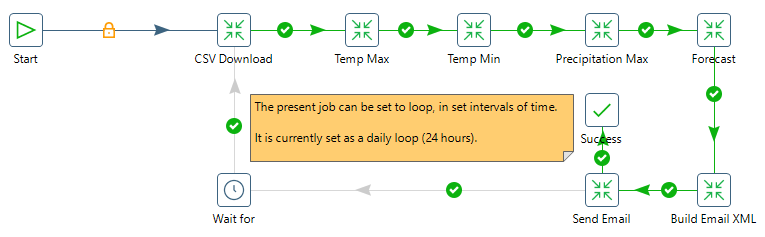
\includegraphics[scale=0.66]{imagens-spoon/job.png}
    \caption{Job Desenvolvido}
\end{figure}

\subsection*{Extração de Informação}

Por motivos de performance, o módulo \textbf{\textit{CSV Input}} não permite o carregamento de um ficheiro CSV utilizando um URL como fonte. 
Assim, de modo a termos acesso à informação necessária, é necessário o download de todos os ficheiros de modo persistente - um total de 14 ficheiros, um por cada concelho do distrito de Braga, disponível na API.

\begin{figure}[H]
    \centering
    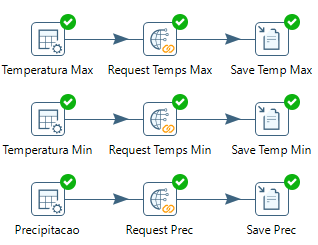
\includegraphics{imagens-spoon/csv_download.png}
    \caption{Transformação \textbf{\textit{CSV Download}}}
\end{figure}

\subsubsection*{Formato dos Ficheiros CSV}

Tendo em conta a estrutura idêntica dos ficheiros de \textbf{Temperatura Máxima}, \textbf{Mínima} e \textbf{Precipitação (Máxima)}, o formato para extração dos dados é igualmente válido para todos.

\begin{figure}[H]
    \centering
    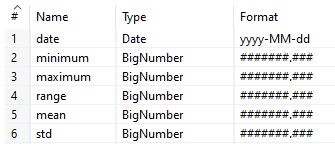
\includegraphics{imagens-spoon/temp-max-fields.png}
    \caption{Formato de Leitura dos Ficheiros CSV descarregados.}
\end{figure}

\begin{figure}[H]
    \centering
    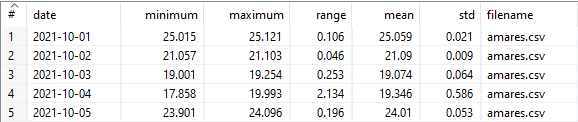
\includegraphics[scale=0.88]{imagens-spoon/temp-max-preview.png}
    \caption{Pré-visualização dos dados dos ficheiros.} 
    {Ex.: Temperatura Máxima}
\end{figure}

A \textbf{\textit{Previsão}} do tempo no entanto, é obtida através de formatação JSON, e pode ser lida através do módulo [\textbf{JSON Input}] utilizando o url correspondente, não sendo necessário o download persistente.

\begin{figure}[H]
    \centering
    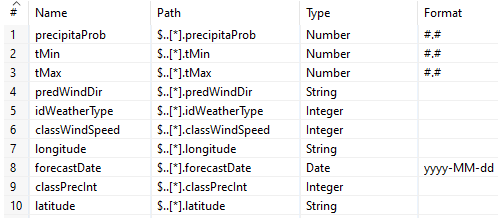
\includegraphics[scale=0.8]{imagens-spoon/previsao-fields.png}
    \caption{Formato de Leitura dos dados JSON. JSON-Path}
\end{figure}

\begin{figure}[H]
    \centering
    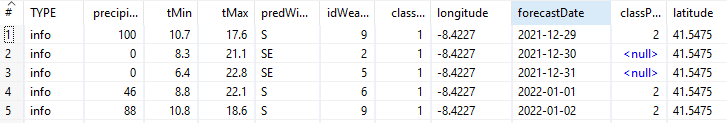
\includegraphics[scale=0.7]{imagens-spoon/previsao-preview.png}
    \caption{Pré-visualização dos dados extraídos.}
\end{figure}

\subsection*{Transformação dos Dados Extraídos}

\begin{figure}[H]
    \centering
    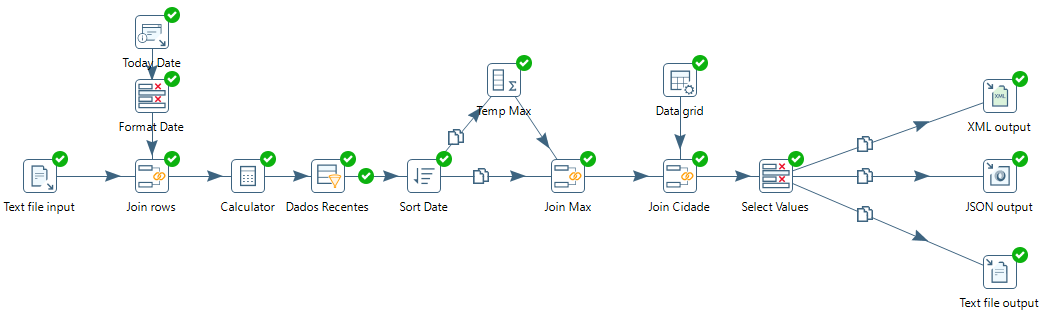
\includegraphics[scale=0.48]{imagens-spoon/temp-max-soon.png}
    \caption{Formato Geral das transformações de um CSV.}
    {Válido para Temp. Máx. e Mín., e Prec. Máx.}
\end{figure}

É utilizado o módulo [\textbf{Text file input}] para que se possa carregar facilmente todos os ficheiros CSV. Infelizmente este método utiliza um caminho completo para o diretório, pelo que se revela uma má solução.

É calculada a diferença entre os dias das informações e o dia atual, recorrendo a informações do sistema, e filtrados aqueles que se encontram no intervalo entre 0 e 10 dias de diferença. São de seguida ordenados por Data e, utilizando o módulo [\textbf{Group By}], é possível encontrar as temperaturas Máximas de cada dia. 

A nova tabela gerada é cruzada com a tabela anterior de modo a reaver os dados perdidos pela operação de Group By.

Por fim, os nomes dos ficheiros são utilizados para atribuir o nome da Cidade correspondente, selecionam-se os dados com informação relevante direcionando-os para os seus outputs: XML, JSON e CSV.

\begin{figure}[H]
    \centering
    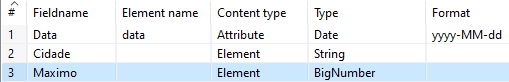
\includegraphics{imagens-spoon/output-pattern.png}
    \caption{Formato XML}
\end{figure}

Os outputs JSON e CSV são bastante simples na sua essência, no entanto o output XML permite algumas alterações como a definição do campo `\textbf{data}' como um atributo do Elemento `\textbf{Day}' do Elemento Raíz `\textbf{Temp-Max/Temp-Min/Prec-Max}'.

Para a informação da \textbf{Previsão} do tempo, são necessárias 3 rotas com informação das classes de: 
\begin{itemize}
    \item Precipitation - Precipitação
    \item Wind - Vento
    \item Weather - Clima
\end{itemize}

Estas rotas retornam informação em formato JSON relativamente a:
\begin{itemize}
    \item Quantidade de Precipitação
    \begin{figure}[H]
        \centering
        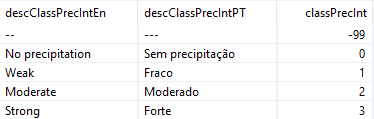
\includegraphics{imagens-spoon/prec-info.png}
    \end{figure}
    \item Força de Vento
    \begin{figure}[H]
        \centering
        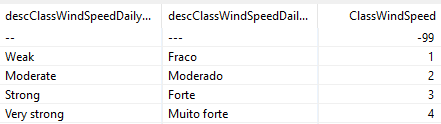
\includegraphics{imagens-spoon/wind-info.png}
    \end{figure}
    \item Estado Meteorológico
    \begin{figure}[H]
        \centering
        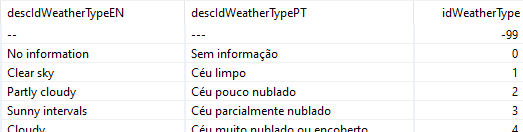
\includegraphics[scale=0.9]{imagens-spoon/weather-info.png}
    \end{figure}
\end{itemize}

Esta informação é cruzada com os id's utilizados nas previsões fornecidas, e posteriormente substituídas por completo por descrições do estado. Este processo é demarcado pelos módulos do tipo [\textbf{Merge Join}].

\begin{figure}[H]
    \centering
    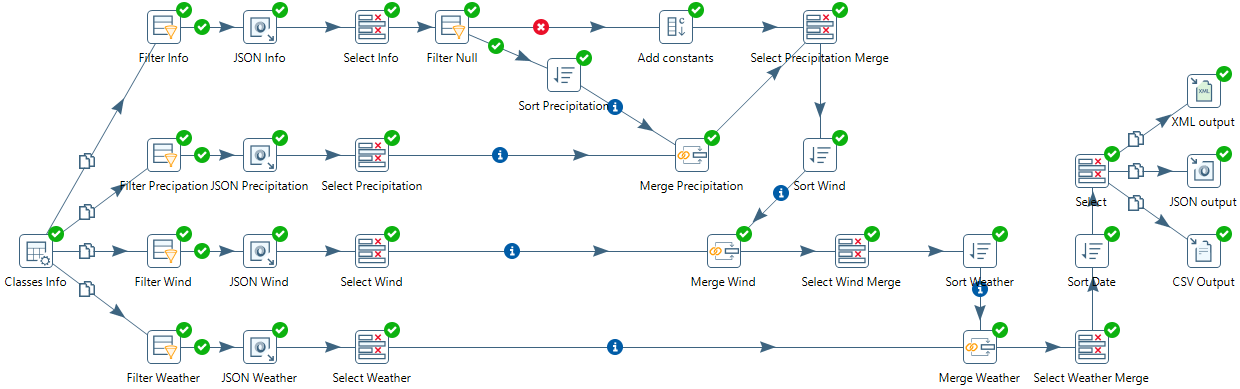
\includegraphics[scale=0.4]{imagens-spoon/previsao-spoon.png}
    \caption{Formato XML}
\end{figure}

Como alguns campos da coluna `\textbf{classPrecInt}' podem ser \textit{null}, nesses casos, são adicionadas as colunas da tabela de informações da classe de Precipitação com valores `\textbf{N/A}'.

\newpage

\subsection*{Envio de Dados para Email}

Utilizando uma base de dados, e uma página HTML construída previamente com as informações a fornecer, são definidos os campos necessários para o envio do email (\textit{sender} email e \textit{password}, \textit{server} e server \textit{port} e ainda o assunto, \textit{subject}, do email).

\begin{figure}[H]
    \centering
    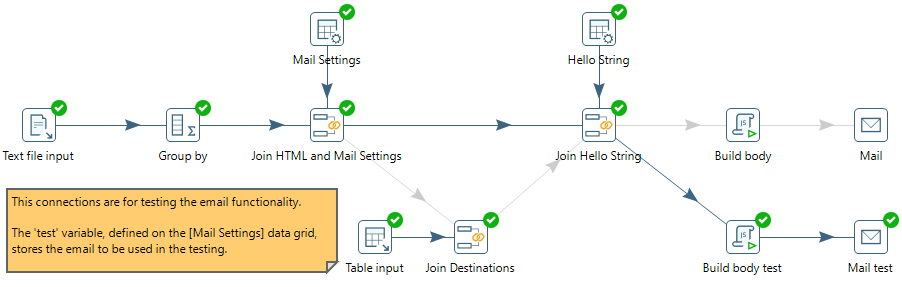
\includegraphics[scale=0.5]{imagens-spoon/email.png}
    \caption{Carregamento de página HTML e envio por email.}
    \label{fig:my_label}
\end{figure}

\subsubsection{Construção de página HTML}

Criando uma \textit{template} XSL, é possível utilizar um ficheiro XML com a informação desejada para criar uma página HTML com tabelas visuais dos Dados.

Para tal é necessário agregar os dados previamente gerados num único XML.

\begin{figure}[H]
    \centering
    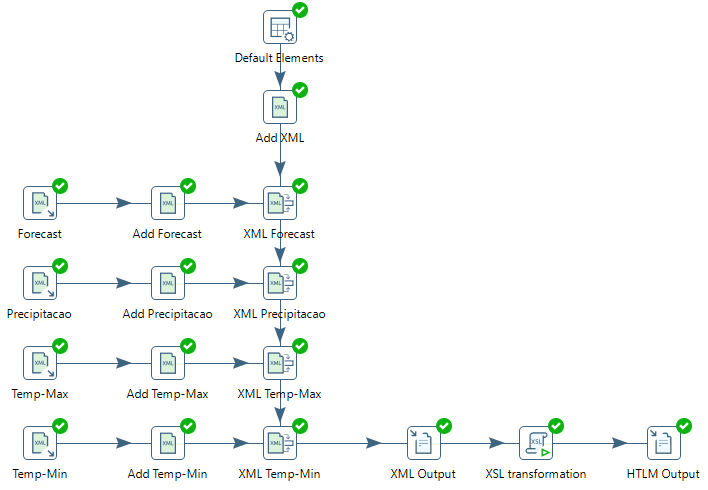
\includegraphics[scale=0.6]{imagens-spoon/html.png}
    \caption{Construção de página HTML utilizando XSL.}
\end{figure}


\newpage